\documentclass{article}%
\usepackage[T1]{fontenc}%
\usepackage[utf8]{inputenc}%
\usepackage{lmodern}%
\usepackage{textcomp}%
\usepackage{lastpage}%
\usepackage[head=40pt,margin=0.5in,bottom=0.6in]{geometry}%
\usepackage{graphicx}%
%
\title{\textbf{12 colegios privados han cerrado sus puertas en Nueva Esparta}}%
\author{EL NACIONAL WEB}%
\date{30/11/2018}%
%
\begin{document}%
\normalsize%
\maketitle%
\textbf{URL: }%
http://www.el{-}nacional.com/noticias/educacion/colegios{-}privados{-}han{-}cerrado{-}sus{-}puertas{-}nueva{-}esparta\_261655\newline%
%
\textbf{Periodico: }%
EN, %
ID: %
261655, %
Seccion: %
Educación\newline%
%
\textbf{Palabras Claves: }%
Educación, Crisis económica, Sociedad\newline%
%
\textbf{Derecho: }%
2.1, %
Otros Derechos: %
, %
Sub Derechos: %
2.1.1\newline%
%
\textbf{EP: }%
NO\newline%
\newline%
%
\textbf{\textit{El aumento de salarios y crisis económica en general ha afectado a varias instituciones privadas en la Isla de Margarita}}%
\newline%
\newline%
%
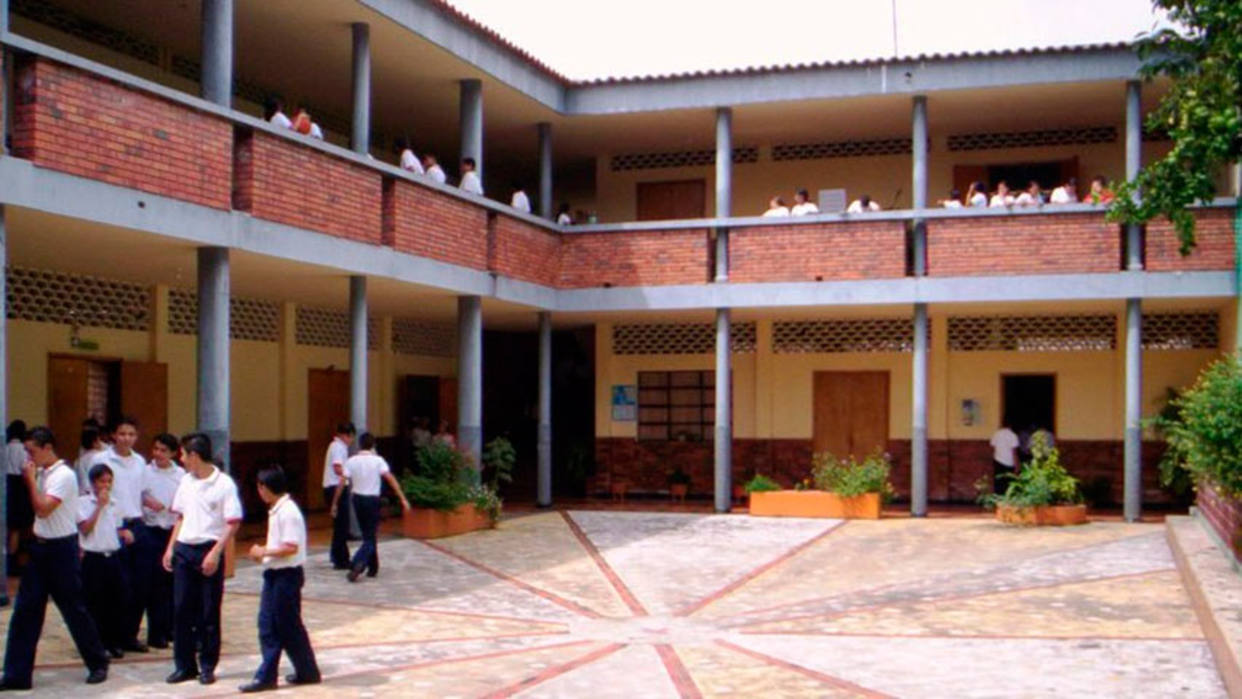
\includegraphics[width=300px]{142.jpg}%
\newline%
%
Yanet López, asesora de la Asociación Nacional de Institutos Educativos Privados, informó que los constantes aumentos salariales han generado crisis en los planteles privados la Isla de Margarita, en Nueva Esparta, donde algunos ya han cerrado sus puertas debido a esta situación.%
\newline%
%
López indicó a~Unión Radio~que actualmente hay un total de 12 colegios que no pudieron dar inicio al año escolar 2018 – 2019. Asimismo, aseguró que aunque algunas instituciones se han mantenido, deben realizarse esfuerzos permanentes para mantenerlas operativas.%
\newline%
%
Por otra parte, la asesora resaltó que hay padres y representantes que han brindado su apoyo para la continuidad de la educación en las aulas y denunció que, tras los desajustes económicos, se han descuidado las infraestructuras de los planteles.%
\newline%
%
Con información de~Unión Radio.%
\newline%
%
\end{document}